% Options for packages loaded elsewhere
\PassOptionsToPackage{unicode}{hyperref}
\PassOptionsToPackage{hyphens}{url}
%
\documentclass[
]{article}
\usepackage{amsmath,amssymb}
\usepackage{lmodern}
\usepackage{ifxetex,ifluatex}
\ifnum 0\ifxetex 1\fi\ifluatex 1\fi=0 % if pdftex
  \usepackage[T1]{fontenc}
  \usepackage[utf8]{inputenc}
  \usepackage{textcomp} % provide euro and other symbols
\else % if luatex or xetex
  \usepackage{unicode-math}
  \defaultfontfeatures{Scale=MatchLowercase}
  \defaultfontfeatures[\rmfamily]{Ligatures=TeX,Scale=1}
\fi
% Use upquote if available, for straight quotes in verbatim environments
\IfFileExists{upquote.sty}{\usepackage{upquote}}{}
\IfFileExists{microtype.sty}{% use microtype if available
  \usepackage[]{microtype}
  \UseMicrotypeSet[protrusion]{basicmath} % disable protrusion for tt fonts
}{}
\makeatletter
\@ifundefined{KOMAClassName}{% if non-KOMA class
  \IfFileExists{parskip.sty}{%
    \usepackage{parskip}
  }{% else
    \setlength{\parindent}{0pt}
    \setlength{\parskip}{6pt plus 2pt minus 1pt}}
}{% if KOMA class
  \KOMAoptions{parskip=half}}
\makeatother
\usepackage{xcolor}
\IfFileExists{xurl.sty}{\usepackage{xurl}}{} % add URL line breaks if available
\IfFileExists{bookmark.sty}{\usepackage{bookmark}}{\usepackage{hyperref}}
\hypersetup{
  pdftitle={Getting Started},
  pdfauthor={Nicole Tresvalles},
  hidelinks,
  pdfcreator={LaTeX via pandoc}}
\urlstyle{same} % disable monospaced font for URLs
\usepackage[margin=1in]{geometry}
\usepackage{color}
\usepackage{fancyvrb}
\newcommand{\VerbBar}{|}
\newcommand{\VERB}{\Verb[commandchars=\\\{\}]}
\DefineVerbatimEnvironment{Highlighting}{Verbatim}{commandchars=\\\{\}}
% Add ',fontsize=\small' for more characters per line
\usepackage{framed}
\definecolor{shadecolor}{RGB}{248,248,248}
\newenvironment{Shaded}{\begin{snugshade}}{\end{snugshade}}
\newcommand{\AlertTok}[1]{\textcolor[rgb]{0.94,0.16,0.16}{#1}}
\newcommand{\AnnotationTok}[1]{\textcolor[rgb]{0.56,0.35,0.01}{\textbf{\textit{#1}}}}
\newcommand{\AttributeTok}[1]{\textcolor[rgb]{0.77,0.63,0.00}{#1}}
\newcommand{\BaseNTok}[1]{\textcolor[rgb]{0.00,0.00,0.81}{#1}}
\newcommand{\BuiltInTok}[1]{#1}
\newcommand{\CharTok}[1]{\textcolor[rgb]{0.31,0.60,0.02}{#1}}
\newcommand{\CommentTok}[1]{\textcolor[rgb]{0.56,0.35,0.01}{\textit{#1}}}
\newcommand{\CommentVarTok}[1]{\textcolor[rgb]{0.56,0.35,0.01}{\textbf{\textit{#1}}}}
\newcommand{\ConstantTok}[1]{\textcolor[rgb]{0.00,0.00,0.00}{#1}}
\newcommand{\ControlFlowTok}[1]{\textcolor[rgb]{0.13,0.29,0.53}{\textbf{#1}}}
\newcommand{\DataTypeTok}[1]{\textcolor[rgb]{0.13,0.29,0.53}{#1}}
\newcommand{\DecValTok}[1]{\textcolor[rgb]{0.00,0.00,0.81}{#1}}
\newcommand{\DocumentationTok}[1]{\textcolor[rgb]{0.56,0.35,0.01}{\textbf{\textit{#1}}}}
\newcommand{\ErrorTok}[1]{\textcolor[rgb]{0.64,0.00,0.00}{\textbf{#1}}}
\newcommand{\ExtensionTok}[1]{#1}
\newcommand{\FloatTok}[1]{\textcolor[rgb]{0.00,0.00,0.81}{#1}}
\newcommand{\FunctionTok}[1]{\textcolor[rgb]{0.00,0.00,0.00}{#1}}
\newcommand{\ImportTok}[1]{#1}
\newcommand{\InformationTok}[1]{\textcolor[rgb]{0.56,0.35,0.01}{\textbf{\textit{#1}}}}
\newcommand{\KeywordTok}[1]{\textcolor[rgb]{0.13,0.29,0.53}{\textbf{#1}}}
\newcommand{\NormalTok}[1]{#1}
\newcommand{\OperatorTok}[1]{\textcolor[rgb]{0.81,0.36,0.00}{\textbf{#1}}}
\newcommand{\OtherTok}[1]{\textcolor[rgb]{0.56,0.35,0.01}{#1}}
\newcommand{\PreprocessorTok}[1]{\textcolor[rgb]{0.56,0.35,0.01}{\textit{#1}}}
\newcommand{\RegionMarkerTok}[1]{#1}
\newcommand{\SpecialCharTok}[1]{\textcolor[rgb]{0.00,0.00,0.00}{#1}}
\newcommand{\SpecialStringTok}[1]{\textcolor[rgb]{0.31,0.60,0.02}{#1}}
\newcommand{\StringTok}[1]{\textcolor[rgb]{0.31,0.60,0.02}{#1}}
\newcommand{\VariableTok}[1]{\textcolor[rgb]{0.00,0.00,0.00}{#1}}
\newcommand{\VerbatimStringTok}[1]{\textcolor[rgb]{0.31,0.60,0.02}{#1}}
\newcommand{\WarningTok}[1]{\textcolor[rgb]{0.56,0.35,0.01}{\textbf{\textit{#1}}}}
\usepackage{graphicx}
\makeatletter
\def\maxwidth{\ifdim\Gin@nat@width>\linewidth\linewidth\else\Gin@nat@width\fi}
\def\maxheight{\ifdim\Gin@nat@height>\textheight\textheight\else\Gin@nat@height\fi}
\makeatother
% Scale images if necessary, so that they will not overflow the page
% margins by default, and it is still possible to overwrite the defaults
% using explicit options in \includegraphics[width, height, ...]{}
\setkeys{Gin}{width=\maxwidth,height=\maxheight,keepaspectratio}
% Set default figure placement to htbp
\makeatletter
\def\fps@figure{htbp}
\makeatother
\setlength{\emergencystretch}{3em} % prevent overfull lines
\providecommand{\tightlist}{%
  \setlength{\itemsep}{0pt}\setlength{\parskip}{0pt}}
\setcounter{secnumdepth}{-\maxdimen} % remove section numbering
\ifluatex
  \usepackage{selnolig}  % disable illegal ligatures
\fi

\title{Getting Started}
\author{Nicole Tresvalles}
\date{8/19/2021}

\begin{document}
\maketitle

Lab documents will be written in R Markdown. This is an R Markdown
document. There are three components of this document that we will pay
attention to in this file:

\begin{enumerate}
\def\labelenumi{\arabic{enumi}.}
\tightlist
\item
  the YAML header at the top of the document
\item
  the Markdown syntax used throughout the document
\item
  the executable code blocks interspersed throughout this document
\end{enumerate}

\hypertarget{yaml-header}{%
\subsection{YAML Header}\label{yaml-header}}

R Markdown documents begin with a YAML header. This is the text that you
see between the `---' (lines 1-6 of this document). This header includes
a number of key-value pairs that provide metadata about the document
(such as its title, who created it, when it was last updated, and the
format in which it should be published). There are certain keys that
appear by default in R Markdown files (e.g.~title, author, date,
output). Depending on the output format you specify, there may be
additional options (such as whether your document should have a table of
contents and how figures should be sized by default).

\begin{quote}
Checkpoint 1: Add your name as the author of this document by editing
the YAML header where it says to ADD YOUR NAME. Be sure to keep the
quotation marks around your name.
\end{quote}

\begin{quote}
After successfully completing checkpoint 1, commit your code (see
instructions in Readme).
\end{quote}

For this research, we will sometimes publish Markdown files as HTML
documents (web documents) and sometimes as PDF documents. To compile
this .Rmd file as one of these documents, we need to `knit' the file.
You can knit this document, but clicking the `Knit' button in the
taskbar above. This document is currently set to output as an HTML file.
We know this because in the YAML header, the `output' key is followed by
the value `html\_document'.

\begin{quote}
Checkpoint 2: Click `Knit' in the taskbar above. A new window will open
with this document formatted as an HTML document. Change the output from
html\_document to pdf\_document. Click `Knit' again. Notice how the
output changes.
\end{quote}

\begin{quote}
After successfully completing checkpoint 2, commit your code again.
\end{quote}

\hypertarget{markdown}{%
\subsection{Markdown}\label{markdown}}

Markdown is a mark-up language - or a computer language that we can use
to communicate to a digital system how we want text and images displayed
when it is published. When you type text into software like Microsoft
Word, you can change the size and font, add bullets, and insert images
by clicking on buttons in the text editor, and the changes are
immediately visible. Markdown is different. To format and style text in
Markdown, we use certain designated symbols and syntax.

For instance, let's say we want to create a heading in our document. To
do this we would add a `\#' and a space in front of the text of our
header like this: (note that Heading One will be the largest text, and
subsequent headings will be increasingly smaller)

\hypertarget{heading-one}{%
\section{Heading One}\label{heading-one}}

\hypertarget{heading-two}{%
\subsection{Heading Two}\label{heading-two}}

\hypertarget{heading-three}{%
\subsubsection{Heading Three}\label{heading-three}}

\hypertarget{heading-four}{%
\paragraph{Heading Four}\label{heading-four}}

\hypertarget{heading-five}{%
\subparagraph{Heading Five}\label{heading-five}}

Heading Six

If we want to add bullets to an R Markdown file, we can add asterisks
(*) and a space in front of the text we want bulletted:

\begin{itemize}
\tightlist
\item
  Bullet one
\item
  Bullet two
\item
  Bullet three
\end{itemize}

If we want to add a hyper-link to an R Markdown file, we can place the
text we want hyper-linked in brackets `{[}{]}' and the link in
parentheses `()' immediately following the bracketed text:

\href{https://github.com/Critical-Data-Analysis-Group}{This is a link to
our GitHub organization.}

Section 3 of
\href{https://www.rstudio.com/wp-content/uploads/2015/02/rmarkdown-cheatsheet.pdf}{this
Cheatsheet} provides a more comprehensive list of syntax rules for R
Markdown.

\begin{quote}
Checkpoint 3: Format the capitalized text immediately below this set of
instructions as \textbf{bold} text. Then knit the document to check how
the text gets displayed in your published document.
\end{quote}

\begin{quote}
After successfully completing checkpoint 3, commit your code again.
\end{quote}

Make \textbf{THIS TEXT} bold.

\hypertarget{code-chunks}{%
\subsection{Code chunks}\label{code-chunks}}

R Markdown documents can include chunks of code and their output. R code
chunks are designated by starting a line with
`\texttt{\{r\}\textquotesingle{}\ and\ ending\ a\ line\ with\ \textquotesingle{}}'.
See below.

\begin{Shaded}
\begin{Highlighting}[]
\NormalTok{sum }\OtherTok{\textless{}{-}} \DecValTok{2} \SpecialCharTok{+} \DecValTok{2}

\NormalTok{sum}
\end{Highlighting}
\end{Shaded}

\begin{verbatim}
## [1] 4
\end{verbatim}

RStudio makes it easy for you to add a code chunk to a document by
clicking the green button +C button in the taskbar and clicking R.

By default when you publish a document with a code chunk, both the code
block and the output of the code will be displayed in the document. If
you add `echo = FALSE' between the leading curly brackets of the code
chunk (following `r'), only the output of the code will be displayed.
The code that created that output will be hidden.

\begin{verbatim}
## [1] 4
\end{verbatim}

Section 5 of
\href{https://www.rstudio.com/wp-content/uploads/2015/02/rmarkdown-cheatsheet.pdf}{this
Cheatsheet} lists other options we can set for code chunks.

\begin{quote}
Checkpoint 4: Add a code chunk below. Copy and paste the following code
and place it in the code chunk: plot(cars) Referencing the linked
cheatsheet, set the figure width to 3 and the figure height to 3. (You
will need to separate these options with a comma.) `Knit' the document
to see how your plot renders in the document.
\end{quote}

\begin{Shaded}
\begin{Highlighting}[]
\FunctionTok{plot}\NormalTok{(cars)}
\end{Highlighting}
\end{Shaded}

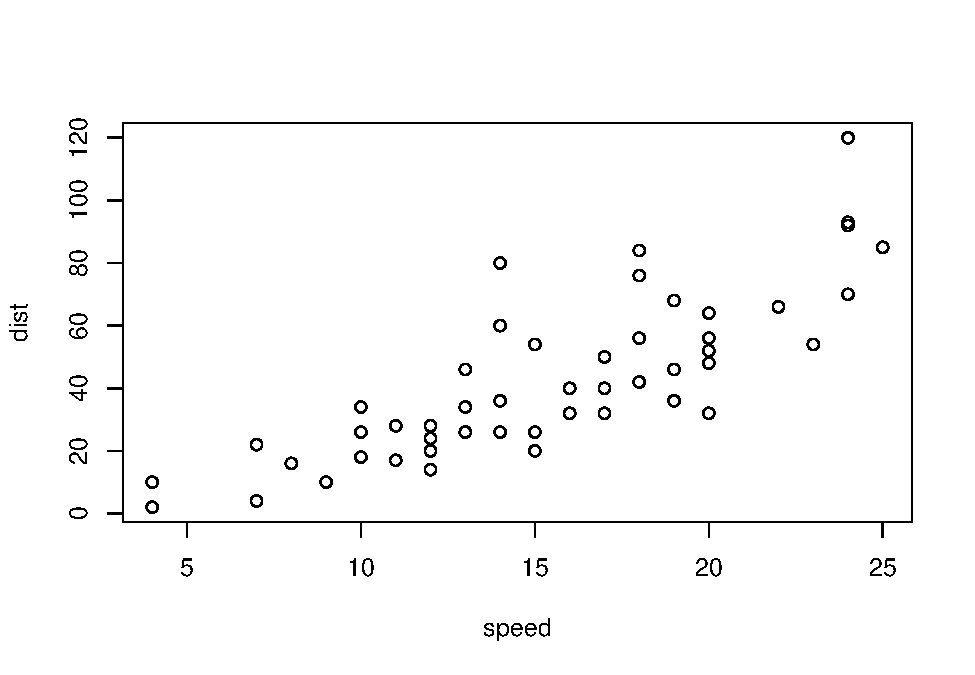
\includegraphics{getting-started-nicole_files/figure-latex/unnamed-chunk-3-1.pdf}

\begin{Shaded}
\begin{Highlighting}[]
\NormalTok{fig.width}\OtherTok{=} \DecValTok{3}
\NormalTok{fig.height}\OtherTok{=} \DecValTok{3}
\end{Highlighting}
\end{Shaded}

\begin{quote}
Stage, commit, and push your code following instructions on GitHub.
\end{quote}

\end{document}
